% Supplementary material (generated tables, see scripts/make_paper_assets.py; figures from ../figures).
\documentclass[conference,onecolumn]{IEEEtran}
\usepackage[T1]{fontenc}
\usepackage{amsmath,amssymb}
\usepackage{graphicx}
\usepackage{booktabs}
\graphicspath{{../figures/}{figures/}}
\renewcommand{\thetable}{S\arabic{table}}
\renewcommand{\thefigure}{S\arabic{figure}}
% Generated by scripts/make_paper_assets.py from results/ - do not edit by hand.
\providecommand{\xspace}{}
\newcommand{\NRawPlayers}{50{,}149}
\newcommand{\NRawValuations}{656{,}301}
\newcommand{\NRawAppearances}{1{,}894{,}350}
\newcommand{\NRawTransfers}{175{,}165}
\newcommand{\NTransfersFee}{17{,}554}
\newcommand{\NValRowsLeakPeriod}{536{,}158}
\newcommand{\NValRowsNoTransfer}{207{,}325}
\newcommand{\PctValRowsNoTransfer}{38.7}
\newcommand{\PctNoTransferIsToday}{100}
\newcommand{\PctTransferIsTransfer}{100}
\newcommand{\PctContractFuture}{54.6}
\newcommand{\NCoreLeagues}{14}
\newcommand{\NNewLeagues}{17}
\newcommand{\CoreLeagueList}{BE1, DK1, ES1, FR1, GB1, GR1, IT1, L1, NL1, PO1, RU1, SC1, TR1, UKR1}
\newcommand{\NRows}{357{,}624}
\newcommand{\NPlayers}{35{,}897}
\newcommand{\NCoreRows}{136{,}653}
\newcommand{\NCorePlayers}{20{,}288}
\newcommand{\NTrain}{112{,}775}
\newcommand{\NVal}{11{,}711}
\newcommand{\NTest}{12{,}167}
\newcommand{\NTestPlayers}{6{,}292}
\newcommand{\NTune}{99{,}976}
\newcommand{\NNewLeagueRows}{8{,}671}
\newcommand{\NLeakChecks}{100}
\newcommand{\NLeakPassed}{100}
\newcommand{\NFeatures}{50}
\newcommand{\NUnknownRows}{76{,}130}
\newcommand{\NUnknownTest}{59}
\newcommand{\BaseRose}{35.4}
\newcommand{\BaseFell}{51.5}
\newcommand{\BaseSame}{13.0}
\newcommand{\MAENaive}{0.480}
\newcommand{\WithinNaive}{32.2}
\newcommand{\MdAPENaive}{37.5}
\newcommand{\MAERidge}{0.407}
\newcommand{\WithinRidge}{35.0}
\newcommand{\MdAPERidge}{30.5}
\newcommand{\SkillRidge}{15.1}
\newcommand{\RhoRidge}{0.56}
\newcommand{\PRiseRidge}{68.8}
\newcommand{\PFallRidge}{90.6}
\newcommand{\RsqChangeRidge}{0.32}
\newcommand{\VsCurveRidge}{3.6}
\newcommand{\MAERF}{0.400}
\newcommand{\WithinRF}{35.8}
\newcommand{\MdAPERF}{29.5}
\newcommand{\SkillRF}{16.6}
\newcommand{\RhoRF}{0.59}
\newcommand{\PRiseRF}{69.8}
\newcommand{\PFallRF}{96.5}
\newcommand{\RsqChangeRF}{0.36}
\newcommand{\VsCurveRF}{5.3}
\newcommand{\MAEXGB}{0.395}
\newcommand{\WithinXGB}{37.3}
\newcommand{\MdAPEXGB}{28.5}
\newcommand{\SkillXGB}{17.7}
\newcommand{\RhoXGB}{0.58}
\newcommand{\PRiseXGB}{71.7}
\newcommand{\PFallXGB}{95.2}
\newcommand{\RsqChangeXGB}{0.35}
\newcommand{\VsCurveXGB}{6.5}
\newcommand{\MAECat}{0.395}
\newcommand{\WithinCat}{37.6}
\newcommand{\MdAPECat}{28.1}
\newcommand{\SkillCat}{17.7}
\newcommand{\RhoCat}{0.58}
\newcommand{\PRiseCat}{72.1}
\newcommand{\PFallCat}{95.7}
\newcommand{\RsqChangeCat}{0.34}
\newcommand{\VsCurveCat}{6.6}
\newcommand{\MAELGB}{0.394}
\newcommand{\WithinLGB}{37.8}
\newcommand{\MdAPELGB}{28.1}
\newcommand{\SkillLGB}{17.9}
\newcommand{\RhoLGB}{0.58}
\newcommand{\PRiseLGB}{73.0}
\newcommand{\PFallLGB}{95.6}
\newcommand{\RsqChangeLGB}{0.33}
\newcommand{\VsCurveLGB}{6.8}
\newcommand{\MAEGRU}{0.397}
\newcommand{\WithinGRU}{37.8}
\newcommand{\MdAPEGRU}{28.2}
\newcommand{\SkillGRU}{17.2}
\newcommand{\RhoGRU}{0.57}
\newcommand{\PRiseGRU}{72.6}
\newcommand{\PFallGRU}{93.5}
\newcommand{\RsqChangeGRU}{0.33}
\newcommand{\VsCurveGRU}{6.0}
\newcommand{\MAEEns}{0.393}
\newcommand{\WithinEns}{38.0}
\newcommand{\MdAPEEns}{27.8}
\newcommand{\SkillEns}{18.1}
\newcommand{\RhoEns}{0.59}
\newcommand{\PRiseEns}{73.4}
\newcommand{\PFallEns}{95.0}
\newcommand{\RsqChangeEns}{0.34}
\newcommand{\VsCurveEns}{7.0}
\newcommand{\MAECurve}{0.423}
\newcommand{\WithinCurve}{35.3}
\newcommand{\MdAPECurve}{31.3}
\newcommand{\SkillCurve}{12.0}
\newcommand{\RhoCurve}{0.51}
\newcommand{\PRiseCurve}{63.6}
\newcommand{\PFallCurve}{92.6}
\newcommand{\RsqChangeCurve}{0.24}
\newcommand{\VsCurveLGBCI}{[6.0, 7.6]}
\newcommand{\VsCurveXGBCI}{[5.7, 7.4]}
\newcommand{\VsCurveCatCI}{[5.7, 7.4]}
\newcommand{\VsCurveRidgeCI}{[2.8, 4.3]}
\newcommand{\VsCurveRFCI}{[4.4, 6.2]}
\newcommand{\VsCurveGRUCI}{[5.1, 7.0]}
\newcommand{\SkillCurveCI}{[10.9, 13.0]}
\newcommand{\SkillLGBCI}{[16.8, 19.0]}
\newcommand{\SkillMomentum}{$-$33.3}
\newcommand{\SkillMomentumDamped}{$-$0.2}
\newcommand{\VsCurveLeagueCurve}{$-$0.2}
\newcommand{\VsCurveLeagueCurveCI}{[$-$0.7, 0.2]}
\newcommand{\MAEeurNaive}{2.89}
\newcommand{\MAEeurLGB}{2.45}
\newcommand{\RsqLevelNaive}{0.83}
\newcommand{\RsqLevelLGB}{0.89}
\newcommand{\GRUsd}{0.003}
\newcommand{\GRUepochs}{9}
\newcommand{\DiffLGBCurve}{$-$0.0286}
\newcommand{\DiffLGBCurveCI}{[$-$0.0322, $-$0.0250]}
\newcommand{\DiffLGBCat}{$-$0.0008}
\newcommand{\DiffLGBCatCI}{[$-$0.0018, 0.0002]}
\newcommand{\DiffLGBXGB}{$-$0.0010}
\newcommand{\DiffLGBXGBCI}{[$-$0.0022, 0.0002]}
\newcommand{\DiffCatXGB}{$-$0.0002}
\newcommand{\DiffCatXGBCI}{[$-$0.0015, 0.0012]}
\newcommand{\DiffLGBGRU}{$-$0.0033}
\newcommand{\DiffLGBGRUCI}{[$-$0.0053, $-$0.0013]}
\newcommand{\DiffLGBEns}{0.0009}
\newcommand{\DiffLGBEnsCI}{[$-$0.0001, 0.0020]}
\newcommand{\DiffLGBRF}{$-$0.0061}
\newcommand{\DiffLGBRFCI}{[$-$0.0087, $-$0.0035]}
\newcommand{\DiffLGBRidge}{$-$0.0135}
\newcommand{\DiffLGBRidgeCI}{[$-$0.0161, $-$0.0107]}
\newcommand{\SplitSkillTime}{17.1}
\newcommand{\SplitMAETime}{0.398}
\newcommand{\SplitSkillRows}{19.7}
\newcommand{\SplitMAERows}{0.359}
\newcommand{\SplitSkillPlayers}{17.5}
\newcommand{\SplitMAEPlayers}{0.373}
\newcommand{\SplitSkillRowsRecent}{23.8}
\newcommand{\SplitSkillPlayersRecent}{19.7}
\newcommand{\LeakLater}{82}
\newcommand{\LeakExact}{47}
\newcommand{\SplitDiffRowsTime}{2.6}
\newcommand{\SplitDiffRowsTimeCI}{[1.0, 4.3]}
\newcommand{\SplitDiffPlayersTime}{0.4}
\newcommand{\SplitDiffPlayersTimeCI}{[$-$1.2, 2.0]}
\newcommand{\SplitDiffRowsPlayers}{2.2}
\newcommand{\SplitDiffRowsPlayersCI}{[1.0, 3.4]}
\newcommand{\SplitDiffRowsTimeRecent}{6.7}
\newcommand{\SplitDiffRowsTimeRecentCI}{[3.8, 9.5]}
\newcommand{\SplitDiffPlayersTimeRecent}{2.6}
\newcommand{\SplitDiffPlayersTimeRecentCI}{[$-$0.6, 5.8]}
\newcommand{\SplitDiffRowsPlayersRecent}{4.1}
\newcommand{\SplitDiffRowsPlayersRecentCI}{[0.4, 7.8]}
\newcommand{\SkillAgeU}{17}
\newcommand{\SkillAgeA}{7}
\newcommand{\SkillAgeB}{15}
\newcommand{\SkillAgeC}{45}
\newcommand{\WithinAgeUNaive}{27.5}
\newcommand{\WithinAgeULGB}{21.8}
\newcommand{\SkillGK}{11}
\newcommand{\SkillCheap}{15}
\newcommand{\SkillExpensive}{20}
\newcommand{\MAEBigFallNaive}{0.66}
\newcommand{\MAEBigFallLGB}{0.44}
\newcommand{\MAEBigRiseNaive}{1.01}
\newcommand{\MAEBigRiseLGB}{0.78}
\newcommand{\MAEStableNaive}{0.02}
\newcommand{\MAEStableLGB}{0.19}
\newcommand{\SkillCoreLeagueMin}{8}
\newcommand{\SkillCoreLeagueMax}{29}
\newcommand{\SkillNewLeagueMin}{8}
\newcommand{\SkillNewLeagueMax}{24}
\newcommand{\NewLeagueNegative}{RSK1}
\newcommand{\SkillNewLeaguesLGB}{13.3}
\newcommand{\SkillOtherLGB}{12.2}
\newcommand{\UnknownModel}{CatBoost}
\newcommand{\MAEcoreWithoutUnknown}{0.3948}
\newcommand{\MAEcoreWithUnknown}{0.3948}
\newcommand{\ShapHist}{32}
\newcommand{\ShapClub}{27}
\newcommand{\ShapPlayer}{17}
\newcommand{\ShapPerf}{13}
\newcommand{\ShapTransfers}{10}
\newcommand{\ShapTopFive}{age, the change since the previous valuation, the value relative to the league median, the number of past valuations and the days since the last match}
\newcommand{\ShapFinRankMin}{33}
\newcommand{\ShapFinRankMax}{36}
\newcommand{\SpendTotalValueCorr}{0.91}
\newcommand{\SnapDiff}{0.0011}
\newcommand{\SnapDiffCI}{[0.00003, 0.0021]}
\newcommand{\AblHist}{0.0089}
\newcommand{\AblPerf}{0.0064}
\newcommand{\AblPlayer}{0.0052}
\newcommand{\AblClub}{0.0039}
\newcommand{\AblTransfers}{0.0004}
\newcommand{\AblFin}{0.0006}
\newcommand{\AblHistOnly}{0.0158}
\newcommand{\SkillHistOnly}{14.6}
\newcommand{\RollVsCurveMin}{3.6}
\newcommand{\RollVsCurveMax}{8.6}
\newcommand{\RollVsCurveMean}{5.8}
\newcommand{\RollVsCurveWins}{6}
\newcommand{\RollCurveMin}{6.6}
\newcommand{\RollCurveMax}{12.0}
\newcommand{\RollSkillMin}{11.5}
\newcommand{\RollSkillMax}{17.1}
\newcommand{\RollSkillMean}{14.5}
\newcommand{\RollRidgeMin}{9.7}
\newcommand{\RollRidgeMax}{15.1}
\newcommand{\RollYears}{6}
\newcommand{\RollLGBWins}{6}
\newcommand{\RollTrainFirst}{48{,}312}
\newcommand{\RollTrainLast}{112{,}775}
\newcommand{\UVRose}{73.0}
\newcommand{\UVRoseCI}{[70.2, 75.8]}
\newcommand{\YoungRose}{65.8}
\newcommand{\YoungRoseCI}{[62.8, 69.2]}
\newcommand{\AllRose}{35.4}
\newcommand{\OVFell}{95.6}
\newcommand{\UVSold}{16.4}
\newcommand{\AllSold}{17.3}
\newcommand{\UVFeeRatio}{2.5}
\newcommand{\AllFeeRatio}{0.88}
\newcommand{\YoungFeeRatio}{1.7}
\newcommand{\UVFeeAbove}{70}
\newcommand{\AllFeeAbove}{40}
\newcommand{\YoungFeeAbove}{69}
\newcommand{\UVAge}{20.3}
\newcommand{\GrpVsCurveU}{9.3}
\newcommand{\GrpVsCurveUCI}{[7.1, 11.5]}
\newcommand{\GrpVsCurveA}{6.6}
\newcommand{\GrpVsCurveACI}{[5.5, 7.7]}
\newcommand{\GrpVsCurveB}{6.3}
\newcommand{\GrpVsCurveBCI}{[4.7, 7.8]}
\newcommand{\GrpVsCurveC}{3.5}
\newcommand{\GrpVsCurveCCI}{[1.4, 5.8]}
\newcommand{\GrpVsCurveBigFall}{9.7}
\newcommand{\GrpVsCurveBigFallCI}{[8.4, 11.0]}
\newcommand{\GrpVsCurveModFall}{13.6}
\newcommand{\GrpVsCurveModFallCI}{[11.0, 16.1]}
\newcommand{\GrpVsCurveModRise}{$-$7.3}
\newcommand{\GrpVsCurveModRiseCI}{[$-$11.1, $-$3.8]}
\newcommand{\GrpVsCurveBigRise}{5.4}
\newcommand{\GrpVsCurveBigRiseCI}{[4.0, 6.6]}
\newcommand{\GrpVsCurveCheap}{5.4}
\newcommand{\GrpVsCurveCheapCI}{[4.0, 6.8]}
\newcommand{\GrpVsCurveExpensive}{6.9}
\newcommand{\GrpVsCurveExpensiveCI}{[4.8, 9.2]}
\newcommand{\GrpVsNaiveC}{45.1}
\newcommand{\GrpPosVsCurveMin}{5.8}
\newcommand{\GrpPosVsCurveMax}{7.3}
\newcommand{\CoreLgPosCount}{12}
\newcommand{\CoreLgNeg}{SC1}
\newcommand{\NewLgPosCount}{6}
\newcommand{\NewLgNegCount}{0}
\newcommand{\RankRiseLGB}{73.0}
\newcommand{\RankRiseYoung}{65.8}
\newcommand{\RankRiseDiff}{7.2}
\newcommand{\RankRiseDiffCI}{[4.2, 10.3]}
\newcommand{\RankFallLGB}{95.6}
\newcommand{\RankFallOld}{88.8}
\newcommand{\RankFallDiff}{6.7}
\newcommand{\RankFallDiffCI}{[4.4, 9.0]}
\newcommand{\RankRiseCurve}{63.6}
\newcommand{\FullWinRows}{7{,}409}
\newcommand{\FullWinVsNaive}{19.8}
\newcommand{\FullWinVsNaiveCI}{[18.6, 21.0]}
\newcommand{\FullWinVsCurve}{8.5}
\newcommand{\FullWinVsCurveCI}{[7.6, 9.6]}
\newcommand{\IntCovRaw}{77.6}
\newcommand{\IntCovRawCI}{[76.8, 78.5]}
\newcommand{\IntCovCal}{80.0}
\newcommand{\IntCovCalCI}{[79.2, 80.9]}
\newcommand{\IntWidthCal}{116}
\newcommand{\IntWidthIncrease}{7}
\newcommand{\IntPinballCal}{0.127}
\newcommand{\IntCovCalU}{77.6}
\newcommand{\IntCovCalUCI}{[75.2, 79.8]}
\newcommand{\IntCovCalC}{81.8}
\newcommand{\IntBelowC}{14.8}
\newcommand{\IntAboveC}{3.4}
\newcommand{\IntAboveU}{14.3}
\newcommand{\IntPinballRef}{0.137}
\newcommand{\IntPinballRaw}{0.127}
\newcommand{\NCalRows}{12{,}799}
\newcommand{\FeeRhoLGB}{0.40}
\newcommand{\FeeRhoLGBCI}{[0.35, 0.46]}
\newcommand{\FeeRhoCurve}{0.33}
\newcommand{\FeeRhoCurveCI}{[0.28, 0.39]}
\newcommand{\FeeRhoAge}{0.38}
\newcommand{\FeeRhoAgeCI}{[0.32, 0.43]}
\newcommand{\FeeRhoTrue}{0.57}
\newcommand{\FeeRhoTrueCI}{[0.53, 0.62]}
\newcommand{\FeeRhoDiffCurve}{0.07}
\newcommand{\FeeRhoDiffCurveCI}{[0.03, 0.11]}
\newcommand{\FeeRhoDiffAge}{0.03}
\newcommand{\FeeRhoDiffAgeCI}{[$-$0.01, 0.07]}
\newcommand{\FeeN}{2{,}100}
\newcommand{\FeePlayers}{1{,}121}
\newcommand{\DropRateTest}{25.5}
\newcommand{\DropTest}{2{,}530}
\newcommand{\DropTestComplete}{9{,}939}
\newcommand{\KeptPartial}{4{,}758}
\newcommand{\DropFell}{43}
\newcommand{\DropRose}{34}
\newcommand{\KeptFell}{41}
\newcommand{\KeptRose}{42}
\newcommand{\DropYoungMedian}{0.21}
\newcommand{\KeptYoungMedian}{0.41}
\newcommand{\NewWindowCov}{46.5}
\newcommand{\NewZeroMin}{87.3}
\newcommand{\CoreZeroMin}{4.7}
\newcommand{\NewNoApp}{72}
\newcommand{\NewVsCurve}{4.1}
\newcommand{\NewVsCurveCI}{[3.1, 5.1]}
\newcommand{\NewVsNaive}{13.3}
\newcommand{\NewNoPerfVsCurve}{2.1}
\newcommand{\NewNoPerfVsCurveCI}{[0.9, 3.2]}
\newcommand{\NewCurveVsNaive}{9.6}
\newcommand{\NResultTables}{55}
\newcommand{\NFigures}{15}
\newcommand{\PctTies}{5.3}

% Double-blind switch, read by main.tex and supplement.tex.
% \anonymoustrue  : submission version (no author block at all, no code link)
% \anonymousfalse : camera-ready version (real author block and GitHub link)
\newif\ifanonymous
\anonymoustrue
       % double-blind switch
\begin{document}
\title{Supplementary Material: Forecasting Football Player Market Values One Year Ahead: A Leak-Checked Public Benchmark}
\author{\ifanonymous\else Tasnim Nahar Raisa\fi}
\maketitle

\section*{S1. Data and features}
Table~\ref{tab:data} gives the observations per split, and Table~\ref{tab:features} lists all \NFeatures{} features. Every feature uses only records dated on or before the valuation date $t$. This was verified with the cut-the-future test described in the main paper.
\begin{table}[!h]
\centering
\caption{Observations per split. Main experiments use the 14 core leagues; the extra test sets cover the same test period.}
\label{tab:data}
\footnotesize
\begin{tabular}{lcrr}
\toprule
Split & Valuation date $t$ & Rows & Players \\
\midrule
Train & 2014-07 -- 2023-06 & 112{,}775 & 17{,}938 \\
Validation & 2023-07 -- 2024-06 & 11{,}711 & 5{,}450 \\
Test & 2024-07 -- 2025-07 & 12{,}167 & 6{,}292 \\
Extra: 17 new leagues & 2024-07 -- 2025-07 & 8{,}671 & 5{,}608 \\
Extra: other clubs & 2024-07 -- 2025-07 & 15{,}079 & 9{,}308 \\
Extra: unknown club & 2024-09 -- 2025-06 & 59 & 41 \\
\bottomrule
\end{tabular}
\end{table}

\begin{table}[!h]
\centering
\caption{The 50 features. Every feature uses only records dated on or before the valuation date $t$.}
\label{tab:features}
\scriptsize
\begin{tabular}{llp{11.5cm}}
\toprule
Feature & Group & Description \\
\midrule
\texttt{age} & player & Age in years at t (from date of birth) \\
\texttt{height\_cm} & player & Height in cm (time-invariant) \\
\texttt{position} & player & Main position: Goalkeeper / Defender / Midfield / Attack \\
\texttt{sub\_position} & player & Detailed position, e.g. Centre-Back, Left Winger \\
\texttt{foot} & player & Preferred foot \\
\texttt{is\_foreign} & player & 1 if citizenship differs from the country of the league at t \\
\texttt{log\_value} & value history & log market value at t \\
\texttt{log\_value\_6m\_ago} & value history & log value of the last valuation dated 120-270 days before t \\
\texttt{log\_value\_12m\_ago} & value history & log value of the last valuation dated 300-450 days before t \\
\texttt{growth\_6m} & value history & log\_value - log\_value\_6m\_ago \\
\texttt{growth\_12m} & value history & log\_value - log\_value\_12m\_ago \\
\texttt{log\_max\_value\_so\_far} & value history & Highest log value up to t \\
\texttt{value\_vs\_max} & value history & log\_value - log\_max\_value\_so\_far (0 = at career peak) \\
\texttt{n\_valuations\_so\_far} & value history & Number of valuations up to t \\
\texttt{days\_since\_prev\_valuation} & value history & Days since the previous valuation \\
\texttt{change\_since\_prev\_valuation} & value history & log change since the previous valuation \\
\texttt{years\_since\_first\_valuation} & value history & Years since the first valuation \\
\texttt{matches\_365} & performance & Matches played in the last 365 days (all competitions) \\
\texttt{minutes\_365} & performance & Minutes played in the last 365 days \\
\texttt{goals\_365} & performance & Goals in the last 365 days \\
\texttt{assists\_365} & performance & Assists in the last 365 days \\
\texttt{ga\_per90\_365} & performance & (Goals + assists) per 90 minutes, last 365 days \\
\texttt{yellow\_365} & performance & Yellow cards in the last 365 days \\
\texttt{red\_365} & performance & Red cards in the last 365 days \\
\texttt{league\_matches\_365} & performance & Domestic-league matches in the last 365 days \\
\texttt{league\_minutes\_365} & performance & Domestic-league minutes in the last 365 days \\
\texttt{league\_ga\_per90\_365} & performance & Domestic-league (goals + assists) per 90, last 365 days \\
\texttt{other\_comp\_minutes\_365} & performance & Minutes in cups / European competitions, last 365 days \\
\texttt{minutes\_prev\_365} & performance & Minutes played 365-730 days before t \\
\texttt{minutes\_change} & performance & minutes\_365 - minutes\_prev\_365 \\
\texttt{ga\_per90\_prev\_365} & performance & (Goals + assists) per 90, 365-730 days before t \\
\texttt{days\_since\_last\_appearance} & performance & Days since the last recorded match \\
\texttt{n\_transfers\_so\_far} & transfers & Number of the player's transfers up to t \\
\texttt{days\_since\_last\_transfer} & transfers & Days since the player's last transfer \\
\texttt{log\_last\_transfer\_fee} & transfers & log(1 + fee) of the player's last transfer \\
\texttt{log\_max\_transfer\_fee} & transfers & log(1 + highest fee) ever paid for the player up to t \\
\texttt{club\_known} & club/league & 1 if the club at t is known (from a transfer or match on/before t), else 0 \\
\texttt{league\_t} & club/league & League at t (from the club's league games); OTHER / UNKNOWN otherwise \\
\texttt{club\_log\_spend\_3y} & club/league & log(1 + fees paid by the club) in the last 3 years \\
\texttt{club\_log\_income\_3y} & club/league & log(1 + fees received by the club) in the last 3 years \\
\texttt{club\_net\_spend\_3y\_m} & club/league & Club net transfer spend in the last 3 years (EUR million) \\
\texttt{club\_games\_365} & club/league & Club matches in the data in the last 365 days \\
\texttt{club\_win\_rate\_365} & club/league & Club win rate in the last 365 days \\
\texttt{club\_gd\_per\_game\_365} & club/league & Club goal difference per game, last 365 days \\
\texttt{club\_mean\_log\_value} & club/league & Mean log value of the club's players (latest month-end snapshot) \\
\texttt{club\_log\_total\_value} & club/league & log total squad value (latest month-end snapshot) \\
\texttt{club\_n\_valued\_players} & club/league & Number of valued players at the club (snapshot) \\
\texttt{value\_vs\_club\_mean} & club/league & log\_value - club\_mean\_log\_value \\
\texttt{league\_median\_log\_value} & club/league & Median log value in the player's league (snapshot) \\
\texttt{value\_vs\_league\_median} & club/league & log\_value - league\_median\_log\_value \\
\bottomrule
\end{tabular}
\end{table}


\clearpage
\section*{S2. Additional results}
\begin{itemize}
\item Table~\ref{tab:s-results}: all models and simple baselines, including the age $\times$ value $\times$ league curve, momentum and the LightGBM + GRU average.
\item Table~\ref{tab:s-calibration}: forecast intervals before and after conformal calibration.
\item Table~\ref{tab:s-dropped}: observations kept and dropped.
\item Table~\ref{tab:s-newleagues}: results with and without the performance features in the core and the new leagues.
\end{itemize}
\begin{table}[!h]
\centering
\caption{All models and baselines on the core-league test set (columns as in the main results table of the paper, plus $R^2$ of the change and the MAE in EUR million). Momentum sometimes predicts extreme changes, which explains its very large euro error.}
\label{tab:s-results}
\footnotesize
\resizebox{\textwidth}{!}{\begin{tabular}{lcccccccccc}
\toprule
Model & MAE$_\Delta$ [95\% CI] & \multicolumn{2}{c}{Skill (\%) vs.} & $\rho$ & P@10$\uparrow$ & P@10$\downarrow$ & MdAPE & $\pm$20\%  & $R^2_\Delta$ & MAE \\
 & & no change & curve [95\% CI] & & (\%) & (\%) & (\%) & (\%)  & & (EUR m) \\
\midrule
No change & 0.480 [0.469, 0.491] & -- & $-$13.6 [$-$15.0, $-$12.2] & -- & -- & -- & 37.5 & 32.2 & 0.00 & 2.89 \\
Age $\times$ value curve & 0.423 [0.412, 0.432] & 12.0 & -- & 0.51 & 63.6 & 92.6 & 31.3 & 35.3 & 0.24 & 2.61 \\
Ridge & 0.407 [0.398, 0.416] & 15.1 & 3.6 [2.8, 4.3] & 0.56 & 68.8 & 90.6 & 30.5 & 35.0 & 0.32 & 2.51 \\
Random forest & 0.400 [0.391, 0.409] & 16.6 & 5.3 [4.4, 6.2] & 0.59 & 69.8 & 96.5 & 29.5 & 35.8 & 0.36 & 2.46 \\
XGBoost & 0.395 [0.386, 0.404] & 17.7 & 6.5 [5.7, 7.4] & 0.58 & 71.7 & 95.2 & 28.5 & 37.3 & 0.35 & 2.47 \\
CatBoost & 0.395 [0.385, 0.403] & 17.7 & 6.6 [5.7, 7.4] & 0.58 & 72.1 & 95.7 & 28.1 & 37.6 & 0.34 & 2.44 \\
LightGBM & 0.394 [0.384, 0.403] & 17.9 & 6.8 [6.0, 7.6] & 0.58 & 73.0 & 95.6 & 28.1 & 37.8 & 0.33 & 2.45 \\
GRU (small check) & 0.397 [0.389, 0.406] & 17.2 & 6.0 [5.1, 7.0] & 0.57 & 72.6 & 93.5 & 28.2 & 37.8 & 0.33 & 2.48 \\
Age $\times$ value $\times$ league curve & 0.424 [0.414, 0.433] & 11.8 & $-$0.2 [$-$0.7, 0.2] & 0.50 & 64.1 & 90.0 & 30.7 & 34.7 & 0.25 & 2.64 \\
Momentum & 0.640 [0.622, 0.656] & $-$33.3 & $-$51.4 [$-$55.0, $-$47.9] & 0.41 & 69.1 & 71.6 & 40.4 & 29.4 & -1.17 & 717.53 \\
Momentum, damped ($\times$0.5) & 0.481 [0.469, 0.492] & $-$0.2 & $-$13.8 [$-$15.6, $-$11.8] & 0.41 & 68.5 & 71.6 & 34.5 & 32.7 & -0.06 & 4.77 \\
LightGBM + GRU (average) & 0.393 [0.384, 0.402] & 18.1 & 7.0 [6.2, 7.9] & 0.59 & 73.4 & 95.0 & 27.8 & 38.0 & 0.34 & 2.44 \\
\bottomrule
\end{tabular}}
\end{table}

\begin{table}[!h]
\centering
\caption{80\% forecast intervals before and after conformal calibration (core test 2024/25). Calibration rows: 12{,}799 training observations whose targets fall between July 2023 and June 2024, i.e. before the test period, and unseen by the calibrated model.}
\label{tab:s-calibration}
\footnotesize
\begin{tabular}{llcccc}
\toprule
Age & Interval & Coverage (\%) [95\% CI] & Below / above (\%) & Median width (log) & Mean pinball \\
\midrule
all & final model, uncalibrated & 77.6 [76.8, 78.5] & 11.5 / 11.0 & 1.06 & 0.127 \\
all & tuning-row model, uncalibrated & 77.1 [76.3, 78.0] & 12.0 / 10.9 & 1.05 & 0.128 \\
all & B + calibration (overall) & 79.7 [78.9, 80.6] & 10.5 / 9.8 & 1.12 & 0.128 \\
all & B + calibration (by age group) & 80.0 [79.2, 80.9] & 10.4 / 9.6 & 1.13 & 0.127 \\
\midrule
$<$21 & final model, uncalibrated & 74.8 [72.3, 77.1] & 9.5 / 15.7 & 1.68 & 0.205 \\
$<$21 & tuning-row model, uncalibrated & 73.9 [71.4, 76.2] & 9.8 / 16.3 & 1.67 & 0.206 \\
$<$21 & B + calibration (overall) & 76.5 [74.1, 78.7] & 8.5 / 15.1 & 1.74 & 0.205 \\
$<$21 & B + calibration (by age group) & 77.6 [75.2, 79.8] & 8.1 / 14.3 & 1.80 & 0.205 \\
\midrule
30+ & final model, uncalibrated & 81.4 [79.4, 83.2] & 13.9 / 4.8 & 0.84 & 0.088 \\
30+ & tuning-row model, uncalibrated & 81.7 [79.9, 83.5] & 14.9 / 3.4 & 0.86 & 0.090 \\
30+ & B + calibration (overall) & 84.4 [82.5, 86.0] & 13.0 / 2.6 & 0.93 & 0.091 \\
30+ & B + calibration (by age group) & 81.8 [79.9, 83.5] & 14.8 / 3.4 & 0.86 & 0.090 \\
\bottomrule
\end{tabular}
\end{table}

\begin{table}[!h]
\centering
\caption{Observations kept and dropped (14 core leagues, valuation dates from July 2014). A genuine drop has a fully observable 10--14-month window without a valuation in it; data-end drops have no target yet because the data end in June 2026.}
\label{tab:s-dropped}
\footnotesize
\begin{tabular}{lrrrrr}
\toprule
Period & Kept & Kept (window partly & Genuine & Dropped at & Genuine drop \\
 & & after data end) & drops & data end & rate (\%) \\
\midrule
train & 112{,}782 & 0 & 31{,}176 & 0 & 21.7 \\
val & 11{,}711 & 0 & 6{,}417 & 0 & 35.4 \\
test & 7{,}409 & 4{,}758 & 2{,}530 & 17{,}953 & 25.5 \\
all periods & 131{,}902 & 4{,}758 & 40{,}123 & 17{,}953 & 23.3 \\
\bottomrule
\end{tabular}
\end{table}

\begin{table}[!h]
\centering
\caption{Test results with and without the performance features. In the 17 new leagues, on average only 46.5\% of the 365-day window has match data, and 87.3\% of observations show zero minutes (core leagues: 4.7\%).}
\label{tab:s-newleagues}
\footnotesize
\begin{tabular}{llccc}
\toprule
Test set & Model & MAE$_\Delta$ & Skill vs.\ no change (\%) & Skill vs.\ curve (\%) \\
\midrule
14 core leagues & age $\times$ value curve & 0.4226 & 12.0 [10.9, 13.0] & -- \\
14 core leagues & LightGBM (all 50 features) & 0.3940 & 17.9 [16.8, 19.0] & 6.8 [5.9, 7.6] \\
14 core leagues & LightGBM without performance & 0.4004 & 16.6 [15.5, 17.6] & 5.3 [4.4, 6.0] \\
\midrule
17 new leagues & age $\times$ value curve & 0.4046 & 9.6 [8.3, 11.0] & -- \\
17 new leagues & LightGBM (all 50 features) & 0.3880 & 13.3 [12.2, 14.5] & 4.1 [3.1, 5.1] \\
17 new leagues & LightGBM without performance & 0.3961 & 11.5 [10.2, 12.9] & 2.1 [0.9, 3.2] \\
\bottomrule
\end{tabular}
\end{table}


\clearpage
\section*{S3. Additional figures}
\begin{itemize}
\item Fig.~\ref{fig:s-rolling}: the rolling-origin evaluation of the main paper, as a figure.
\item Fig.~\ref{fig:s-league}: the skill of LightGBM per league, against both references.
\item Fig.~\ref{fig:s-intervals}: forecast intervals for 50 random test players.
\item Fig.~\ref{fig:s-uv}: the ``undervalued'' check (value change and later transfers for the 10\% largest predicted rises and falls).
\end{itemize}

\begin{figure}[!h]
\centering
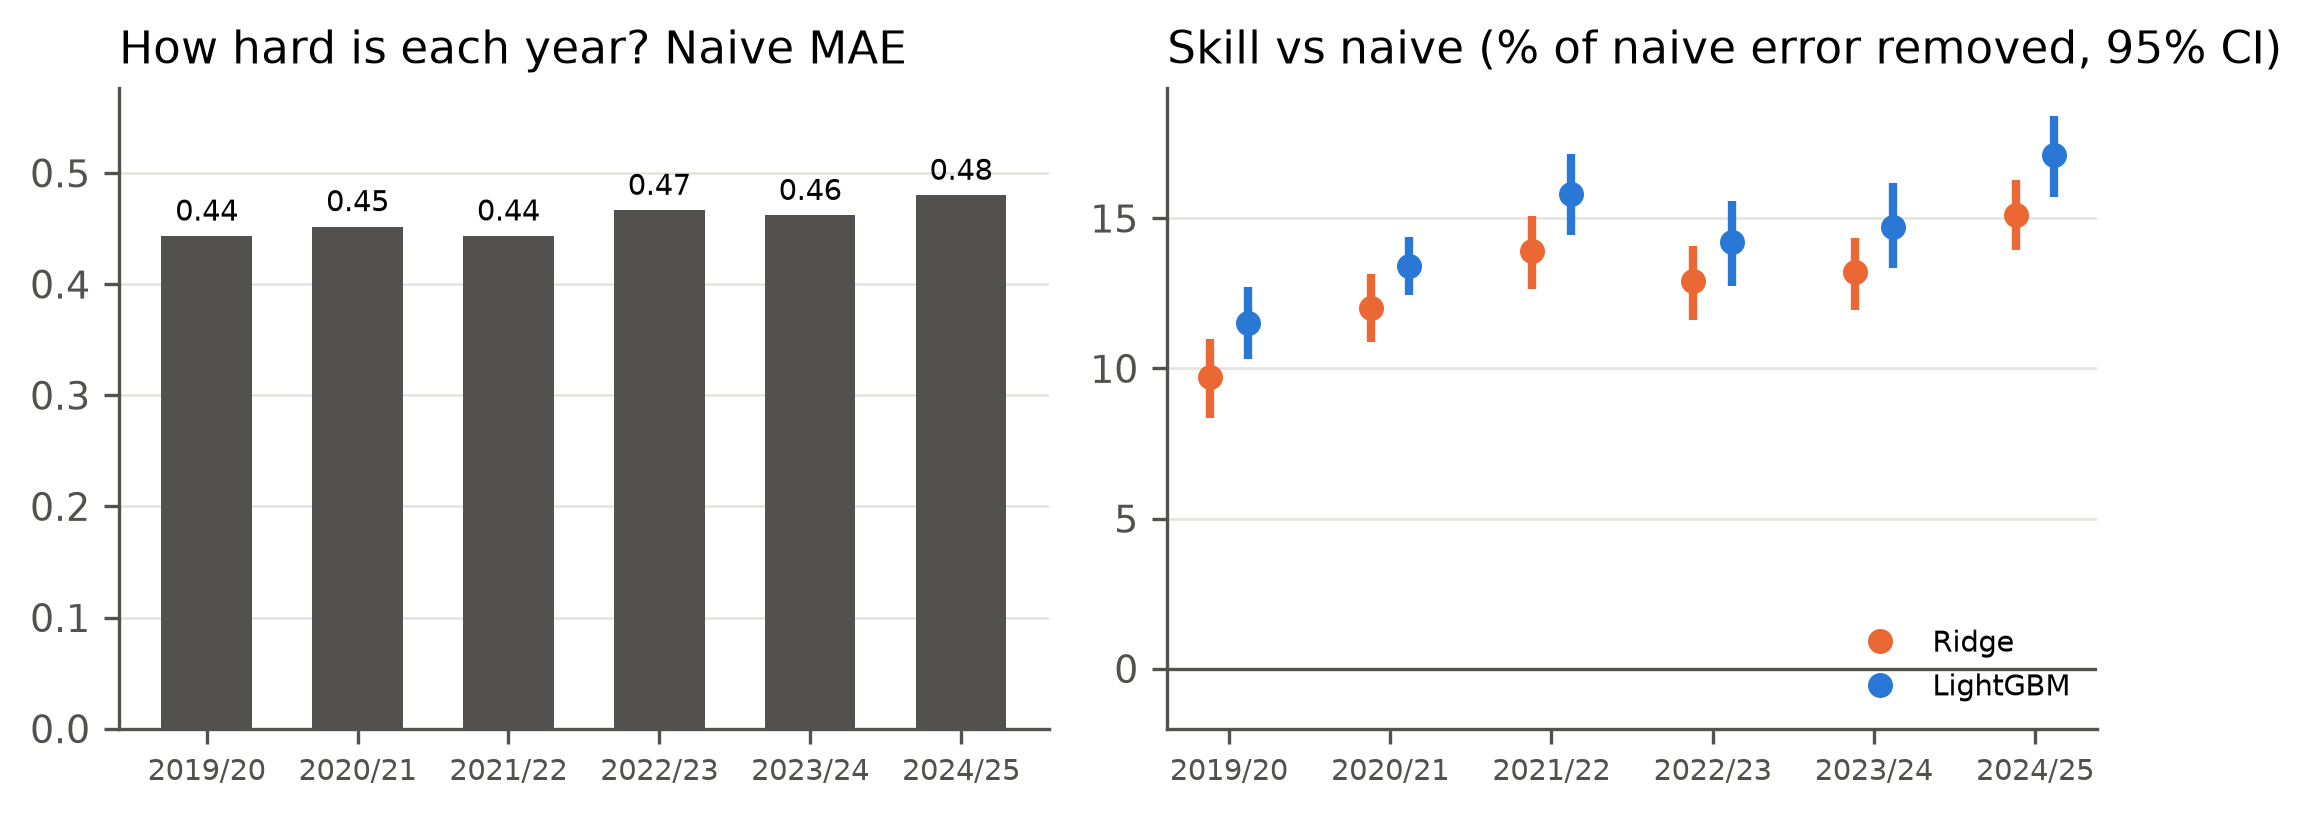
\includegraphics[width=0.75\textwidth]{fig13_rolling_origin.png}
\caption{Rolling-origin evaluation. Left: error of the no-change forecast per test year. Right: skill against no change of the age $\times$ value curve, ridge and LightGBM, with 95\% player-level bootstrap intervals.}
\label{fig:s-rolling}
\end{figure}

\begin{figure}[!h]
\centering
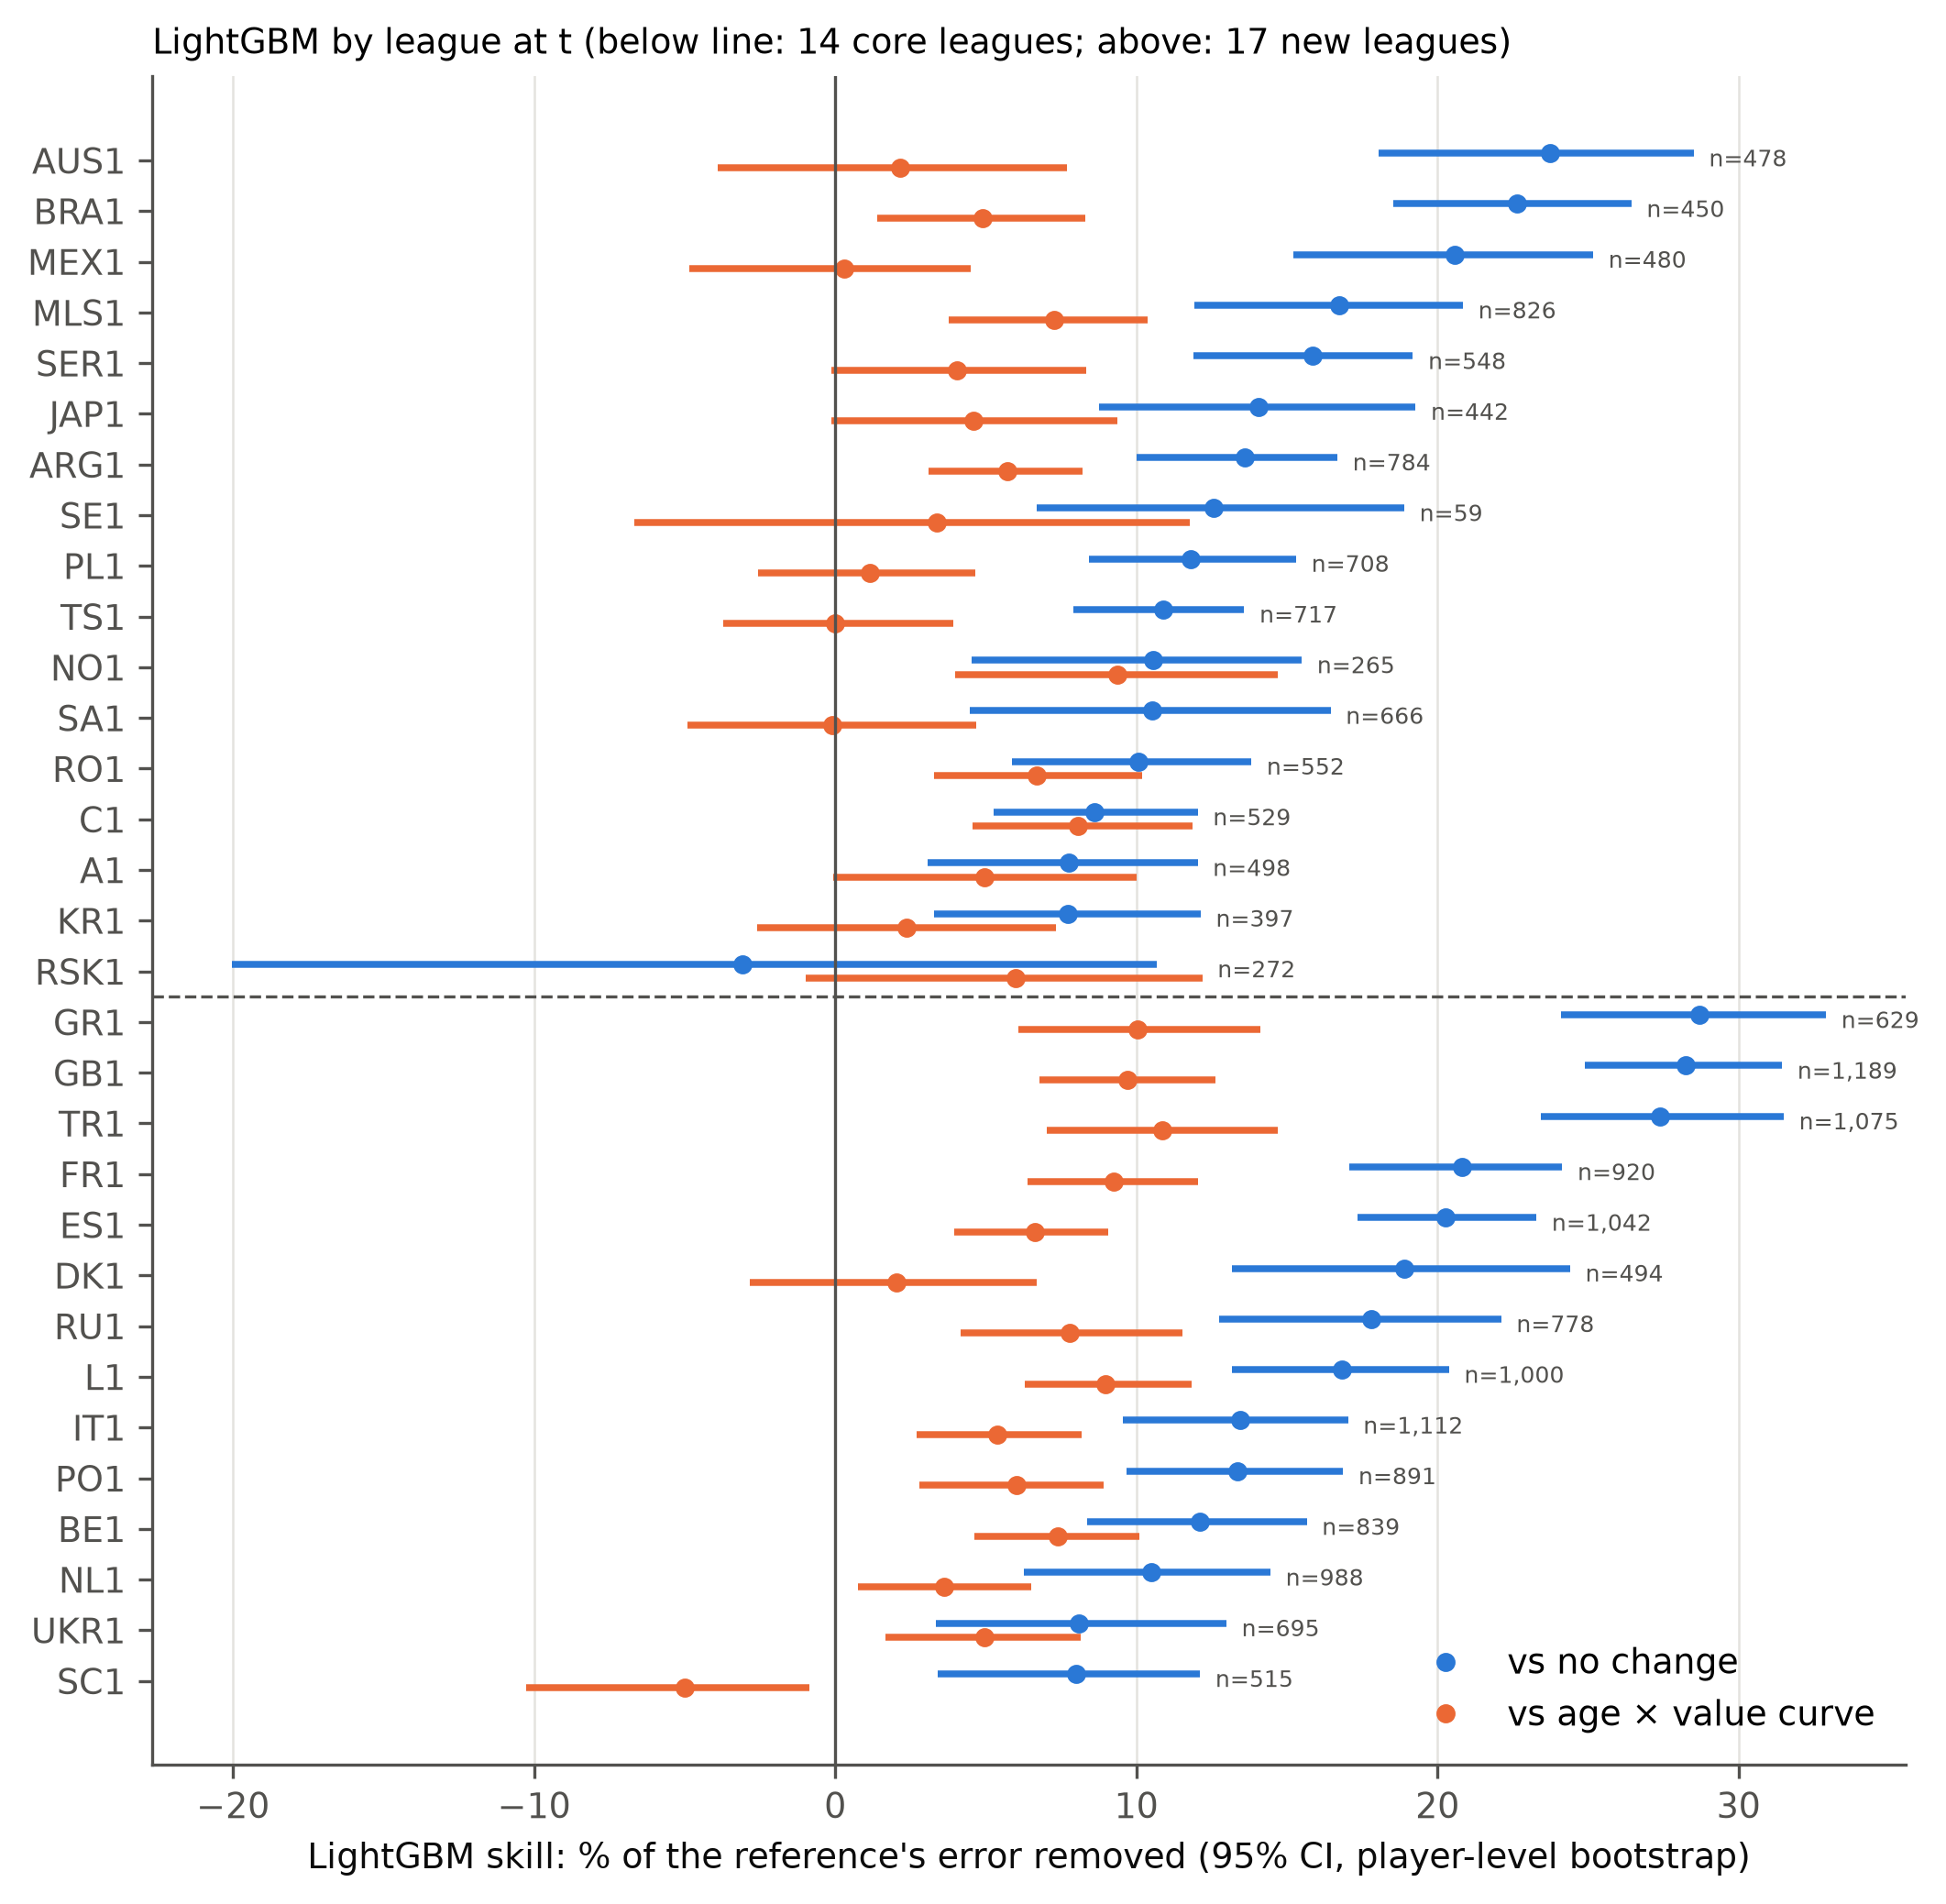
\includegraphics[width=0.6\textwidth]{fig08_gain_by_league.png}
\caption{LightGBM skill by league at $t$ (test period), against no change and against the age $\times$ value curve, with 95\% player-level bootstrap intervals. Below the dashed line: the 14 core leagues used for training; above: the 17 new leagues.}
\label{fig:s-league}
\end{figure}

\begin{figure}[!h]
\centering
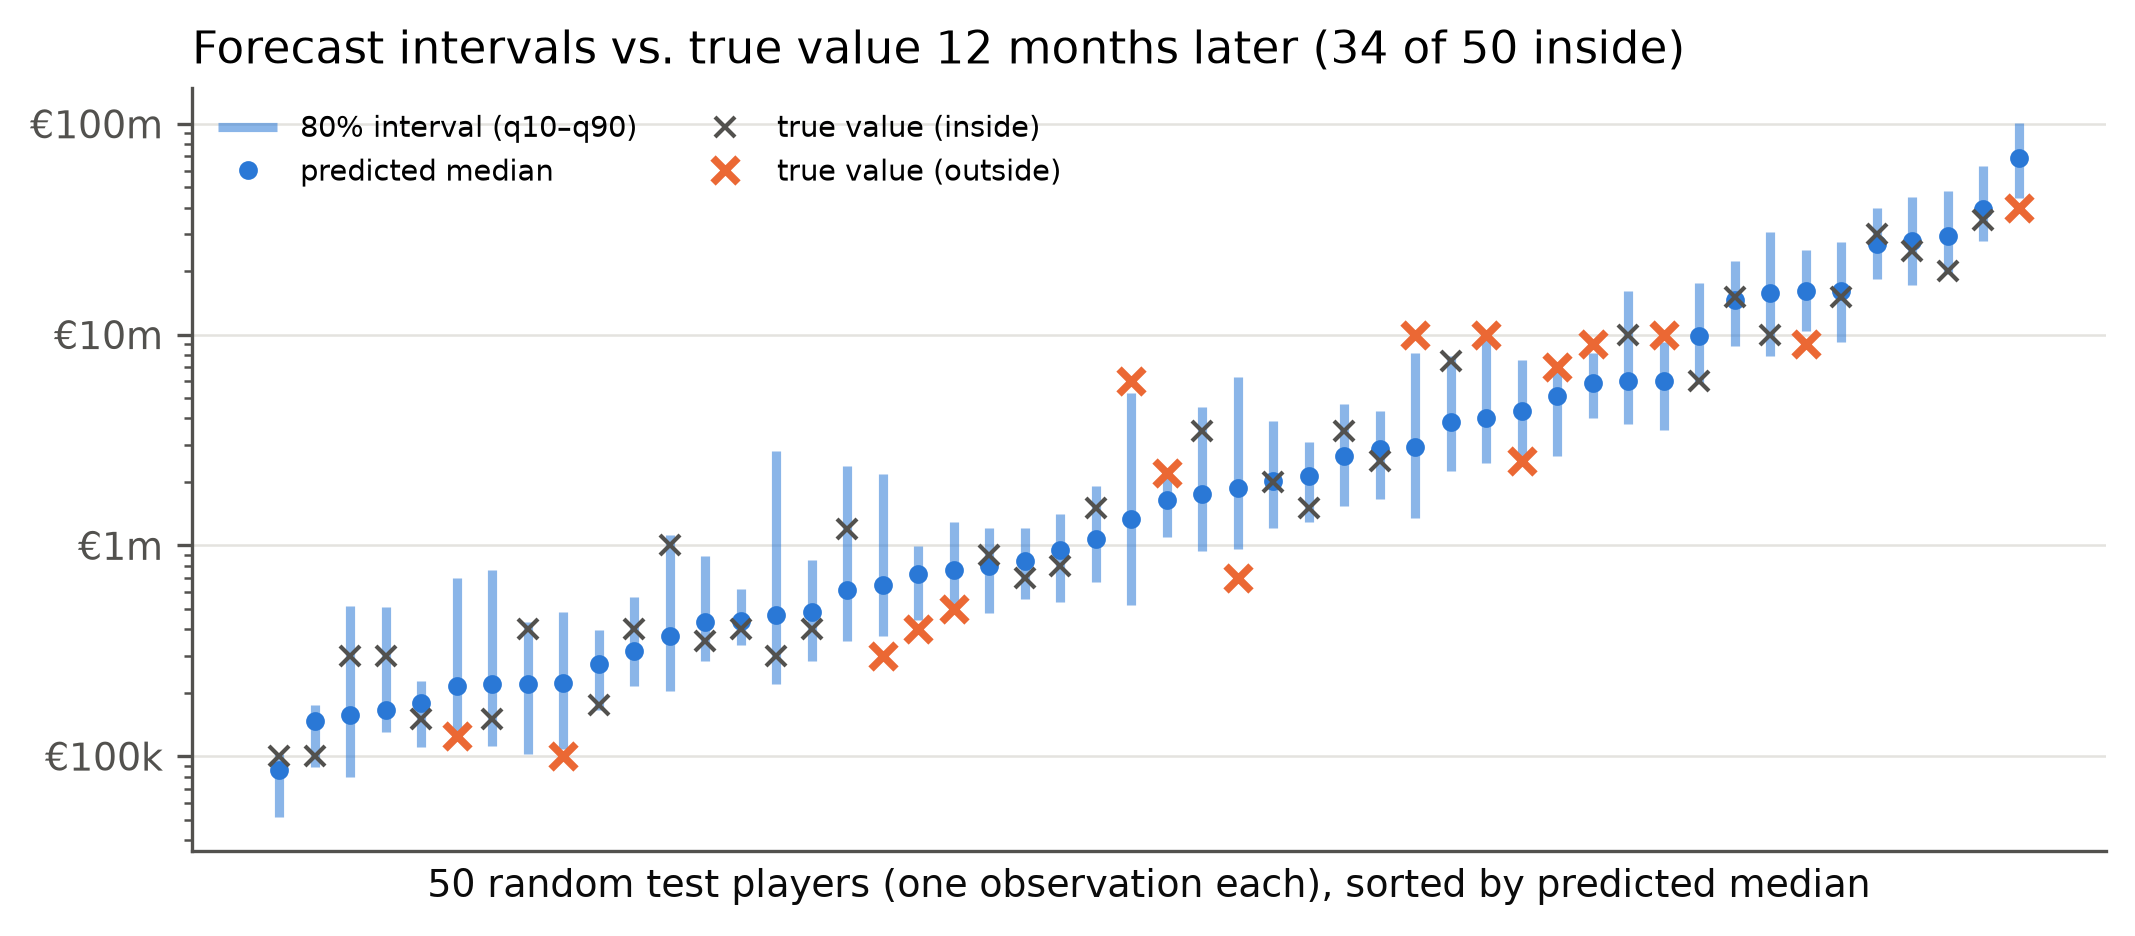
\includegraphics[width=0.8\textwidth]{fig15_forecast_intervals.png}
\caption{Uncalibrated 80\% forecast intervals (LightGBM quantile models) and true values 12 months later for 50 random test players.}
\label{fig:s-intervals}
\end{figure}

\begin{figure}[!h]
\centering
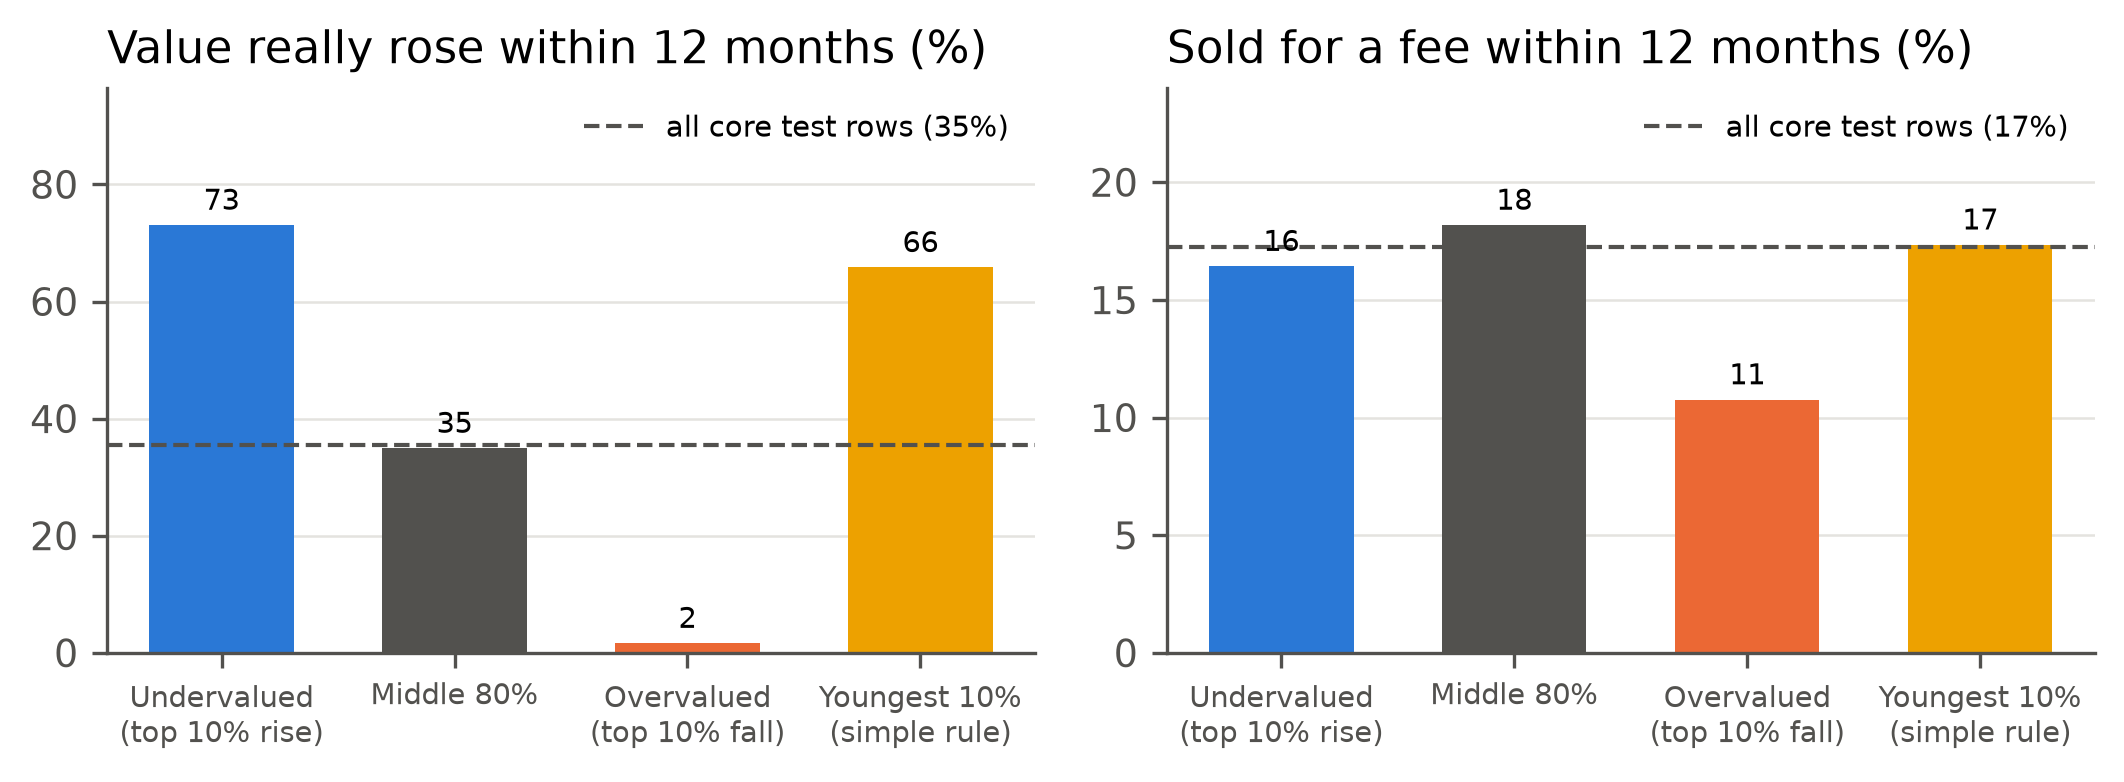
\includegraphics[width=0.75\textwidth]{fig12_undervalued_check.png}
\caption{Share of players whose value rose within 12 months, and share sold for a fee within 12 months: the 10\% largest predicted rises and falls, the middle 80\%, and the youngest 10\%.}
\label{fig:s-uv}
\end{figure}

\end{document}
